\documentclass[11pt]{article}
\usepackage[margin=1in]{geometry}
\usepackage{amsmath,amssymb,amsthm}
\usepackage[T1]{fontenc}
\usepackage{lmodern}
\usepackage{graphicx}
\usepackage[hidelinks]{hyperref}

\newtheorem{theorem}{Theorem}
\newtheorem{lemma}{Lemma}

\title{A Weak-Norm Counterexample to Problem 13.1 in Blei's Grothendieck Inequality Revisited}
\author{Run fa\_banach\_001, agent\_lane\_14}
\date{2026-07-03}

\begin{document}
\maketitle

\section*{Status}

This packet gives a likely valid counterexample to Problem 13.1 in Ron
Blei's ``The Grothendieck inequality revisited'', arXiv:1111.7304.
It proves that both inclusions displayed in (13.1) of the source paper are
proper.

\section*{Source Problem}

The source problem appears in Section 13.1, ``Some loose ends'', on PDF pages
92--93. The displayed inclusions are:

\begin{center}
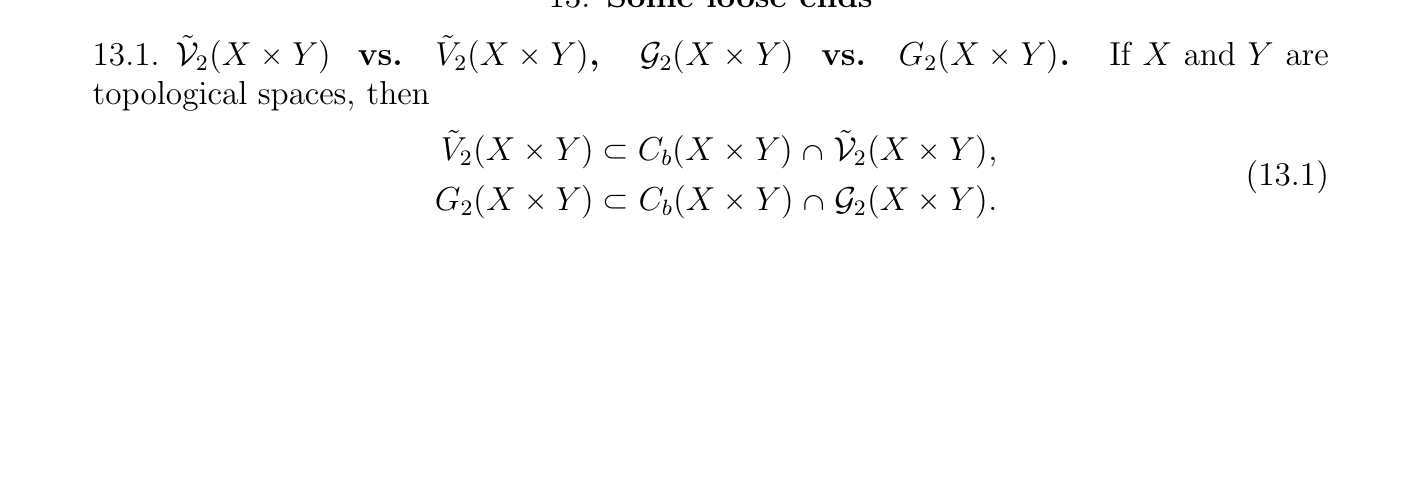
\includegraphics[width=\textwidth]{figures/open_problem_crop_page92.png}
\end{center}

The problem statement is:

\begin{center}
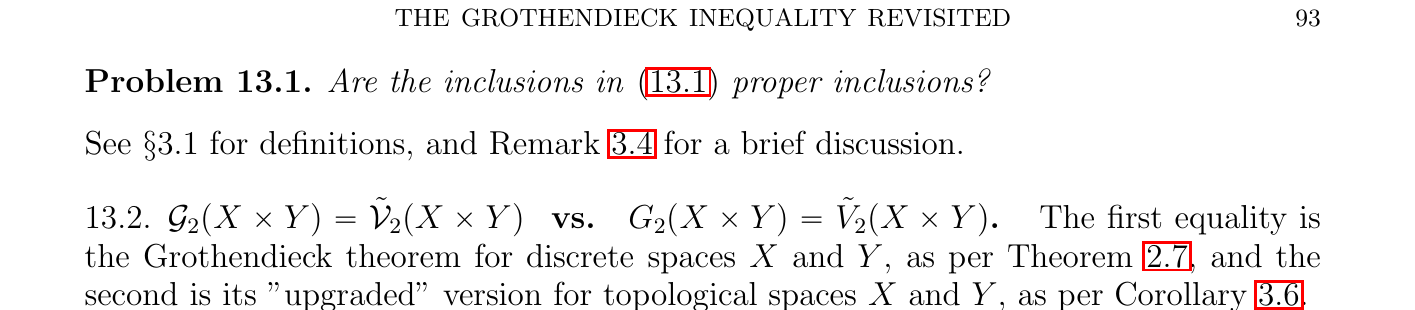
\includegraphics[width=\textwidth]{figures/open_problem_crop_page93.png}
\end{center}

In text form, Problem 13.1 asks whether, for topological spaces \(X\) and \(Y\),
the inclusions
\[
\widetilde V_2(X\times Y)
   \subset C_b(X\times Y)\cap \widetilde{\mathcal V}_2(X\times Y),
\qquad
G_2(X\times Y)
   \subset C_b(X\times Y)\cap \mathcal G_2(X\times Y)
\]
are proper.

\section*{Proof Intuition}

The source's topological classes require Hilbert factorizations whose
coordinate maps are norm-continuous after the given topologies on \(X\) and
\(Y\) are taken into account. The set-theoretic classes forget this continuity.
The unit ball of an infinite-dimensional Hilbert space supplies exactly the
gap: the inner product is jointly continuous for weak topology in the first
variable and norm topology in the second, and it has the obvious set-theoretic
Hilbert factorization. But any topological \(G_2\)-factorization would force
the weak-to-norm identity map on the Hilbert ball to be continuous, which is
ruled out by an orthonormal sequence.

\section*{Counterexample}

\begin{theorem}
Let \(H=\ell^2(\mathbb N)\). Let
\[
X=(B_H,\sigma(H,H^*)),\qquad Y=(B_H,\|\cdot\|)
\]
be the closed unit ball of \(H\), with the weak topology on \(X\) and the norm
topology on \(Y\). Define
\[
f:X\times Y\to \mathbb C,\qquad f(x,y)=\langle x,y\rangle .
\]
Then
\[
f\in C_b(X\times Y)\cap \mathcal G_2(X\times Y)
\]
but \(f\notin G_2(X\times Y)\). Consequently the second inclusion in (13.1) is
proper. Moreover, using the discrete Grothendieck theorem
\(\mathcal G_2=\widetilde{\mathcal V}_2\) and the inclusion
\(\widetilde V_2\subset G_2\) from the source paper, the same \(f\) also shows
that
\[
\widetilde V_2(X\times Y)
\subset C_b(X\times Y)\cap \widetilde{\mathcal V}_2(X\times Y)
\]
is proper.
\end{theorem}

\begin{proof}
The function \(f\) is bounded by \(1\). It is jointly continuous on
\(X\times Y\): if \(x_i\to x\) weakly in \(B_H\) and \(y_i\to y\) in norm, then
\[
|\langle x_i,y_i\rangle-\langle x,y\rangle|
\leq |\langle x_i,y_i-y\rangle|+|\langle x_i-x,y\rangle|
\leq \|y_i-y\|+|\langle x_i-x,y\rangle|\to 0.
\]
Thus \(f\in C_b(X\times Y)\).

As a set-theoretic kernel, \(f\) belongs to \(\mathcal G_2(X\times Y)\), where
the topologies on \(X\) and \(Y\) are ignored. Indeed, put
\(\Omega=\mathbb N\) and \(\mu(\{n\})=2^{-n}\). For
\(x=(x_n),y=(y_n)\in B_H\), define
\[
g_x(n)=2^{n/2}x_n,\qquad h_y(n)=2^{n/2}\overline{y_n}.
\]
Then \(\|g_x\|_{L^2(\mu)}=\|x\|_2\leq 1\) and
\(\|h_y\|_{L^2(\mu)}=\|y\|_2\leq 1\), while
\[
\int_\Omega g_x(\omega)h_y(\omega)\,d\mu(\omega)
=\sum_{n=1}^\infty x_n\overline{y_n}
=f(x,y).
\]

Suppose, toward a contradiction, that \(f\in G_2(X\times Y)\). By Definition
3.2 of the source paper, there are a probability space \((\Omega,\mu)\) and
\(L^2(\mu)\)-continuous maps
\[
g:X\to L^2(\Omega,\mu),\qquad h:Y\to L^2(\Omega,\mu)
\]
such that
\[
f(x,y)=\int_\Omega g(x)(\omega)h(y)(\omega)\,d\mu(\omega)
\]
and
\[
C:=\sup_{x\in X,\;y\in Y}\|g(x)\|_2\|h(y)\|_2<\infty .
\]
Since \(f\) is not identically zero, choose \(x_0\in X\) with \(g(x_0)\ne 0\).
Then
\[
M:=\sup_{y\in Y}\|h(y)\|_2\leq C/\|g(x_0)\|_2<\infty .
\]
For all \(x,x'\in B_H\),
\[
\|x-x'\|
=\sup_{y\in B_H}|\langle x-x',y\rangle|
=\sup_{y\in B_H}|f(x,y)-f(x',y)|
\leq M\|g(x)-g(x')\|_2 .
\]
The map \(g:X\to L^2(\Omega,\mu)\) is continuous from the weak topology on
\(B_H\) to the Hilbert norm topology. The displayed estimate therefore implies
that the identity map
\[
(B_H,\sigma(H,H^*))\longrightarrow (B_H,\|\cdot\|)
\]
is continuous. This is impossible in infinite dimension: if
\((e_n)\) is an orthonormal sequence in \(H\), then \(e_n\to 0\) weakly while
\(\|e_n-0\|=1\) for every \(n\).

Hence \(f\notin G_2(X\times Y)\). Since the source paper proves
\(\widetilde V_2(X\times Y)\subset G_2(X\times Y)\), \(f\notin
\widetilde V_2(X\times Y)\). Also, the source's Theorem 2.7 identifies the
set-theoretic Grothendieck class \(\mathcal G_2\) with
\(\widetilde{\mathcal V}_2\). Therefore \(f\) belongs to the right side of both
inclusions in (13.1) and to neither left side. Both inclusions are proper.
\end{proof}

\section*{Verification and Novelty Notes}

No computation is used. The only functional-analytic input beyond the source
definitions is the elementary fact that an orthonormal sequence in an
infinite-dimensional Hilbert space converges weakly to \(0\) but not in norm.

Bounded novelty search performed before promotion:
\begin{itemize}
\item Run indexes were searched for `1111.7304', `Grothendieck inequality
revisited', `Problem 13.1', `proper inclusions', and close
\(\widetilde V_2/G_2\) phrases. No exact prior packet was found.
\item Local parsed arXiv sources were searched for the exact Problem 13.1
wording and weak-topology/norm-topology variants. No separate answer was
identified.
\item Web searches for the exact Problem 13.1 wording, the source title with
`Problem 13.1', and close \(\widetilde V_2/G_2\) proper-inclusion phrases
returned no direct answer.
\end{itemize}
Novelty confidence is moderate pending human literature review; the proof is
short and self-contained.

\section*{Human Review Recommendation}

Reviewers should check the alignment of notation with Definitions 2.4, 3.2,
Proposition 3.3, Corollary 3.6, and Problem 13.1 of the source paper. In
particular, verify that the explicit representation over
\((\mathbb N,\mu(\{n\})=2^{-n})\) satisfies the source's set-theoretic
\(\mathcal G_2\) definition, while topological \(G_2\) requires \(L^2\)-norm
continuous representing families.

\begin{thebibliography}{9}
\bibitem{Blei}
Ron Blei, \emph{The Grothendieck inequality revisited}, arXiv:1111.7304.
\end{thebibliography}

\end{document}
